\documentclass[nostrict]{szablonPG}

%-------------------- Dodatkowe pakiety ---------------------
% komendy usepackage
\usepackage{multirow}
\usepackage{booktabs}
\usepackage{makecell}
\usepackage{tabularx}
\usepackage{longtable}
\usepackage{listing_schemat}
%------------------------------------------------------------

%------------------------------------------------------------
%			      Poczatek pracy dyplomowej  
%------------------------------------------------------------

\begin{document}

%------------------------------------------------------------
%  Dodanie strony tytulowej wygenerowanej z MojaPG oraz 
%  						oswiadczenia

%\includepdf{meta/strona_tytulowa.pdf}
%\includepdf{meta/oswiadczenie.pdf}

%------------------------------------------------------------
%  Dodanie streszczenia i abstract
%  						

\chapter*{Streszczenie}
\indent W poni�szej pracy opisano etapy budowania platformy edukacyjnej wykorzystuj�cej szeroko poj�te mechanizmy grywalizacji, nazywan� zamiennie gamifikacj�. W pierwszym rozdziale om�wiono wst�p i cel pracy. W drugim rozdziale przedstawiono g��wne mechanizmy grywalizacji oraz tematyk� kursu realizowanego w ramach studium przypadku. W trzecim rozdziale dokonano przegl�du istniej�cych rozwi�za� w obszarze zdalnego nauczania i wykorzystywania mechanizm�w gamifikacji. W kolejnym opisano analiz� projektowanego systemu. Zawarto w nim takie elementy jak wizja systemu, diagramy przypadk�w u�ycia i diagram klas. W pi�tym rozdziale opisano projekt systemu, czyli metodyk� pracy, architektur� ca�ego systemu oraz przedstawiono schemat bazy danych. W sz�stym i si�dmym rozdziale opisano szczeg�y implementacji wybranych fragment�w systemu oraz studium przypadku. W ko�cowym rozdziale przedstawiono wnioski i spostrze�enia w postaci podsumowania.\vspace{0.5cm}\newline

\noindent \textbf{S�owa kluczowe:} gamifikacja, nauczanie zdalne, diagramy UML, serwis internetowy\vspace{0.5cm}\newline
\noindent \textbf{Dziedzina nauki i techniki, zgodnie z wymogami OECD:} Informatyka
\chapter*{Abstract}
\indent The following paper describes the stages of building an educational platform that uses the mechanisms of gamification, interchangeably called gamification. The first chapter discusses the introduction and purpose of the paper. The second chapter presents the main mechanisms of gamification and the subject matter of the case study course. The third chapter reviews existing solutions in the area of remote learning and the use of gamification mechanisms. The next one describes the analysis of the designed system. It includes elements such as system vision, use case diagrams and class diagram. The fifth chapter describes the system design, i.e. the working methodology, the architecture of the whole system, and presents the database schema. The sixth and seventh chapters describe implementation details of selected parts of the system and a case study. The final chapter presents conclusions and insights in the form of a summary. \vspace{0.5cm}\newline

\noindent \textbf{Keywords:} gamification, remote learning, UML diagrams, web service\vspace{0.5cm}\newline
\noindent \textbf{Field of science and technology, as required by the OECD: } Computer Science

%------------------------------------------------------------
%	Utworzenie spisu tresci pracy dyplomowej
\tableofcontents

%------------------------------------------------------------
%	Dodanie wykazu wazniejszych skrotow i oznaczen 
\chapter*{Wykaz wa�niejszych oznacze� i skr�t�w}
\addcontentsline{toc}{chapter}{Wykaz wa�niejszych oznacze� i skr�t�w}

 
API -- Application Programming Interface 

ABI -- Application Binary Interface 


%------------------------------------------------------------
%	Dodanie rozdzialoww pracy dyplomowej - glowne cialo dokumentu 

\chapter{Wst�p i cel pracy}

\chapter{Opis dziedziny problemowej (Krzysztof Sajko)}

\section{Gamifikacja w edukacji}

Gamifikacja bywa te� nazywana grywalizacj� i jest ona u�yciem element�w gier i technik projektowania gier w kontek�cie nie zwi�zanymi z grami. Nazwa tego podej�cia pochodzi od tego, �e to przemys� gier by� pionierem w tej dziedzinie, bo gry nie maj� innego celu, ni� zadowolenie osoby w nie graj�cej \cite{deterding}. Wart podkre�lenia jest tutaj fakt, i� gamifikacja w edukacji nie powinna by� rozumiana jako wykorzystanie gier w procesie dydaktycznym. Gamifikacja to raczej metoda, dzi�ki kt�rej zwi�ksza si� zaanga�owanie student�w poprzez obj�cie szerokiego zakresu czynno�ci edukacyjnych, systemem, kt�ry ma motywowa� i jest w du�ej mierze zbli�ony do przebiegu gry. Przyk�adowo podczas prowadzenia gamifikacji na uczelni wy�szej zalecane jest, aby zapewni� studentom \cite{mochocki}

\begin{itemize}
\item kilka �cie�ek do sukcesu (zaliczenia przedmiotu)
\item realn� mo�liwo�� pora�ki (niezaliczenie przedmiotu)
\item stopniowe dawkowanie materia�u w miar� post�p�w
\item istnienie element�w losowych, niespodziewanych
\item przejrzyst� map� kursu, ukazuj�c� powi�zanie zada� z celami kszta�cenia
\item epick� formu�a zada�, role/to�samo�ci i narracj� zbudowan� wok� tematyki zaj�� (studenci jako agenci)
\item informacje zwrotne (przyznawane punkty)
\item listy rankingowe wzmacniaj�ce motywacj�
\end{itemize}

Og�lnie rzecz bior�c gamifikacja jest sposobem projektowania, kt�ry k�adzie du�y nacisk na ludzk� motywacj� w procesie i wykorzystuje wszystkie wci�gaj�ce w rozgrywk� mechanizmy, jakie wyst�puj� w grach \cite{octalysis}. Wi�kszo�� system�w skupia si� na funkcjonalno�ci i przypomina sytuacj�, gdzie pracownicy musz� wykonywa� swoj� prac�, bo s� do niej zobowi�zani. Gamifikacja takiemu podej�ciu przeczy i skupia si� w g��wnej mierze na uczuciach i motywacji korzystaj�cych z systemu os�b. 

Wed�ug bada� przeprowadzonych w�r�d student�w Akademii Marynarki Wojennej, kt�rzy korzystali z platformy zbudowanej specjalnie na potrzeby systemu grywalizacji \cite{rodwald}:
\begin{itemize}
\item �rednia liczba student�w uczestnicz�cych w wyk�adach wynosi�a 82\%, co oznacza wzrost 34\% w stosunku do grupy, dla kt�rej przedmiot odbywa� si� bez wykorzystania gamifikacji
\item �rednia liczba student�w oddaj�ce sprawozdania laboratoryjne w dniu zaj�� wynosi 90\%, co stanowi wzrost o 81\% w stosunku do grupy bazowej
\item �rednia liczba student�w bior�cych udzia� w nieobowi�zkowych zadaniach wynosi 82\%, czyli praktycznie wszyscy, kt�rzy uczestnicz� w wyk�adach
\end{itemize}

\section{Mechanizmy gamifikacji}

Jeden z pionier�w gamifikacji, Yu-kai Chou opracowa� framework, kt�ry ma pom�c w budowaniu system�w korzystaj�cych z jej mechanizm�w. Wyr�ni� on w nim 8 podstawowych filar�w takiego systemu \cite{octalysis}.

% =======================================
% epickie znaczenie

Pierwszym i zarazem najbardziej kluczowym filarem gamifikacji jest tzw. "epickie znaczenie" (ang. \textit{Meaning}). Jest to zasada wedle kt�rej gracz (czy te� ucze�) wierzy, �e robi co� wi�cej ni� zwyk�e zadanie zlecone przez nauczyciela. Osoby, kt�re s� cz�onkami  systemu, kt�ry korzysta z tego mechanizmu robi� to nie dlatego, �e praca w nim przynosi im bezpo�rednie korzy�ci, ale dlatego, �e dzi�ki nim staj� si� bohaterami historii wykreowanej po cz�ci przez system i po cz�ci przez nich samych. Przyk�adowe techniki, kt�re wdra�aj� t� zasad� w �ycie s� przedstawione na rysunku \ref{chapter2_octalyst1}. W�r�d nich na uwag� zas�uguj� szczeg�lnie
\begin{itemize}
\item Narracja (ang. \textit{Narrative}) - wi�kszo�� gier rozpoczyna rozgrywk� od wprowadzenia dlaczego u�ytkownik powinien gra� w t� gr�. Pozwala to wprowadzi� histori�, kt�ra pozwala ludziom zdoby� kontekst, dzi�ki kt�remu s� w stanie nawi�za� lepsz� interakcje z systemem.  
\item Bohater ludzko�ci (ang. \textit{Humanity Hero}) - technika, kt�ra ma powi�za� dzia�ania podj�te przez u�ytkownik�w z faktem, �e maj� one du�y wk�ad w sprawienie, �e �wiat stanie si� lepszym miejscem. Przyk�adowo firma TOM�s Shoes za wykonane u nich zakupy wysy�a jedn� par� but�w dla dzieci z kraj�w trzeciego �wiata, co sprawia �e robi�c zakupy mamy wra�enie, �e pomagamy ludzko�ci.   
\item Elitaryzm (ang. \textit{Elitism}) - jest to technika, w kt�rej pozwala si� u�ytkownikom na tworzenie dumnych grup opartych na pochodzeniu etnicznym, przekonaniach, czy zainteresowaniach. Daje im to wra�enie, �e s� cz�ci� wi�kszej sprawy. Przyk�adem mo�e by� rywalizacja pomi�dzy uniwersytetami.
\end{itemize}

\begin{figure}[H]
	\centering
	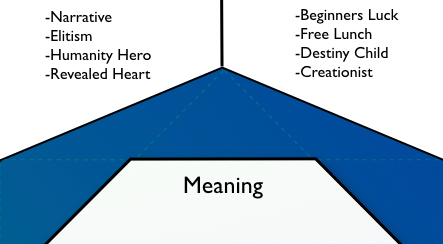
\includegraphics[scale=0.5]{img/chapter2/octalyst1.png}
	\caption{Octalyst - epickie znaczenie \cite{octalysis}}
	\label{chapter2_octalyst1}
\end{figure}

% =======================================
% rozwoj i osiagniecia

Drugim z filar�w grywalizacji jest oparcie systemu o zasad� rozwoju i osi�gni�� (ang. \textit{Accomplishment}). Jest to zasada, kt�ra prawi o tym, �e rozw�j i osi�gni�cia to wewn�trzny nap�d do robienia post�p�w, rozwijania umiej�tno�ci i ostatecznie pokonywania wyzwa�. Kluczowym sformu�owaniem jest tutaj wyzwanie, gdy� s�owo jest bardzo motywuj�ce przy realizacji zada�. W my�l tej zasady powsta�o wiele prostych w realizacji, ale daj�cych ogromne efekty technik, do kt�rych nale�� mi�dzy innymi: zdobywanie punkt�w, ranking lider�w, czy zdobywanie osi�gni�� i nagr�d. Inne przyk�adowe techniki buduj�ce ten filar gamifikacji mo�na zobaczy� na rysunku \ref{chapter2_octalyst2}

\begin{figure}[H]
\centering
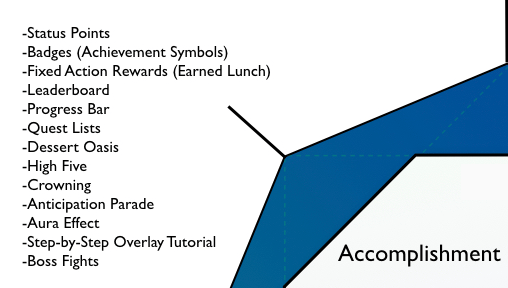
\includegraphics[scale=0.5]{img/chapter2/octalyst2.png}
\caption{Octalyst - rozw�j i osi�gni�cia \cite{octalysis}}
\label{chapter2_octalyst2}
\end{figure}

% =======================================
% wzmocnienie kreatywnosci

Kolejnym filarem wskazanym przez Chou jest wzmocnienie kreatywno�ci (ang.  \textit{Empowerment}). Jest to zasada, kt�rej celem jest zbudowanie sytuacji, w kt�rej u�ytkownicy s� zaanga�owani w proces tw�rczy. Przez to s� zobowi�zani do ci�g�ej pracy, w kt�rej musz� my�le� i tworzy� nowe kombinacje. Nale�y r�wnie� pami�ta�, o tym, �e tak samo jak ludzie maj� potrzeb� wyra�ania swojej kreatywno�ci, tak samo maj� potrzeb� by zobaczy� jej efekty. Techniki pozwalaj�ce wdro�y� te zasady w �ycie mo�na zobaczy� na rysunku \ref{chapter2_octalyst3}, a najbardziej efektywne z nich s�:

\begin{itemize}
\item Boosters - technika ta polega na mo�liwo�ci zdobycia przez gracza jakiego� przedmiotu lub zdolno�ci, kt�ra na chwil� drastycznie zwi�ksza jego umiej�tno�ci. Przyk�adowo mo�e to by� mikstura odporno�ci, kt�ra zapewni odporno�� na wszelkie obra�enia a ci�gu minuty od jej wypicia.  
\item Odblokowanie kamienia milowego - technika ta wykorzystuje mechanizm stosowany w grach RPG polegaj�cy na odblokowywaniu nowych umiej�tno�ci wraz ze zdobyciem nowego poziomu. Przyk�adowo przeciwnicy, kt�rzy do tej pory sprawiali nam trudno��, dzi�ki nowo zdobytej umiej�tno�ci s� �atwi do pokonania
\item Plant Picker - jest to technika, kt�re swoje korzenie ma w grze Plants vs Zombies. W gruncie rzeczy chodzi o to, �e u�ytkownik po odblokowaniu kamieni milowych musi wybra� kilka z nich w nadchodz�cej rozgrywce. W pierwowzorze polega�o to na wybraniu kilku odpowiednich ro�lin, kt�re gracz b�dzie m�g� wykorzysta� w rozgrywce. 
\end{itemize}

\begin{figure}[H]
\centering
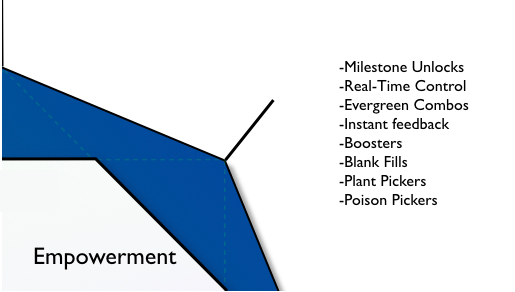
\includegraphics[scale=0.5]{img/chapter2/octalyst3.png}
\caption{Octalyst - wzmocnienie kreatywno�ci \cite{octalysis}}
\label{chapter2_octalyst3}
\end{figure}

% =======================================
% wlasnosc i posiadanie

Czwartym filarem gamifikacji jest idea w�asno�ci i posiadania (ang. \textit{Ownership}). Wed�ug niej u�ytkownicy, kt�rzy s� w�a�cicielami jakich� d�br czuj� si� dobrze w�a�nie dzi�ki temu.  Kiedy gracz jest w�a�cicielem odczuwa pod�wiadomie ch�� sprawienia, by to co posiada sta�o si� lepsze i posiada� co raz wi�cej d�br. Przyk�adowe techniki dzia�aj�ce w ramach tej idei znajduj� si� na rysunku \ref{chapter2_octalys4}, a najbardziej godnymi uwagi s�:

\begin{itemize}
\item Budowanie od podstaw (ang. \textit{Build from Scratch}) - w technice tej wykorzystuje si� zjawisko zwi�kszenia zaanga�owania poprzez mo�liwo�� udzia�u w procesie ju� na wczesnym etapie. Przyk�adem tutaj mog� by� meble firmy IKEA, do kt�rych ludzie wydaj� si� by� bardziej przywi�zani ni� do takich, kt�re s� drogie i robione na zam�wienie. Powodem nie musi by� tutaj ich cena, ale fakt, �e u�ytkownik sk�ada� je samodzielnie. 
\item Zestawy kolekcjonerskie (ang. \textit{Collection sets}) - jest to jedna na najsilniejszych technik gamifikacyjnych i polega na mobilizowaniu gracza do skompletowania pewnego zestawu przedmiot�w, kt�ry zebrany w ca�o�ci daje du�e poczucie warto�ci. Niejednokrotnie s�yszano o sytuacjach, gdzie karty kolekcjonerskie by�y sprzedawane za setki tysi�cy dolar�w
\end{itemize}

\begin{figure}[H]
\centering
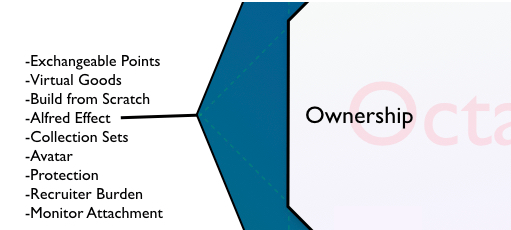
\includegraphics[scale=0.5]{img/chapter2/octalyst4.png}
\caption{Octalyst - w�asno�� i posiadanie \cite{octalysis}}
\label{chapter2_octalys4}
\end{figure}

% =======================================
% relacje i wplyw spoleczny

Kolejnym wa�nym czynnikiem podczas budowania systemu opartego o gamifikacje s� relacje i wp�yw spo�eczny (ang. \textit{Social Influence}). W gamifikacji to mechanizm, kt�ry obejmuje wszystkie elementy spo�eczne, kt�re nap�dzaj� ludzi do dzia�ania. Dotyczy to mi�dzy innymi mentoringu, akceptacji, reakcji spo�ecznych oraz konkurencj� i zazdro��. W�r�d wielu technik (\ref{chapter2_octalyst5}), kt�re s� w tym obr�bie wykorzystywane na uwag� zas�uguj� mi�dzy innymi:

\begin{itemize}
\item Mentoring (ang. \textit{Mentorship}) - technika ta polega na po��czeniu ze sob� osoby do�wiadczonej i nowicjusza. Obie strony czerpi� w�wczas z tej relacji korzy�ci - nowicjusz zyskuje wiedz� i do�wiadczenie oraz �atwiej mu si� odnale�� w nowym �rodowisku. Weteran z kolei zyskuje pomoc w utrzymaniu zaanga�owania w rozgrywce. 
\item Grupowe zadania (ang. \textit{Group Quests}) - technika ta jest bardzo skuteczna w grze zespo�owej, poniewa� wymaga udzia�u grupy, zanim pojedyncza osoba osi�gnie zwyci�stwo. �wietnym przyk�adem jest tutaj gra World of Warcraft, gdzie mamy dost�p do zada�, kt�re wymagaj� udzia�u zespo�u. Zadania te zmobilizowa�y graczy do tworzenia klan�w, w kt�rych regularnie je wykonuj�. 
\end{itemize}
 
\begin{figure}[H]
\centering
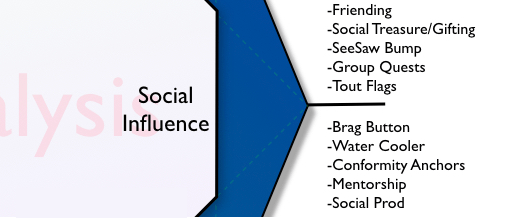
\includegraphics[scale=0.5]{img/chapter2/octalyst5.png}
\caption{Octalyst - relacje spo�eczne \cite{octalysis}}
\label{chapter2_octalyst5}
\end{figure} 
 
% =======================================
% niedostatek i niecierpliwosc
 
Sz�stym ju� z kolei filarem gamifikacji jest zasada niedostatku i niecierpliwo�ci (\textit{Scarcity}). Wykorzystuje ona naturalny ludzki nap�d do posiadania czego�, tylko dlatego, ze nie mo�esz tego mie�. Wiele gier wykorzystuje ten mechanizm poprzez odblokowywania nagr�d dopiero po pewnym czasie. Fakt tego, �e nagrod� otrzymamy, ale nie w tym momencie silnie motywuje ludzi i sprawia, �e s� w stanie my�le� o niej przez ca�y dzie�. Przyk�adowe techniki (\ref{chapter2_octalyst6}) to:

\begin{itemize}
\item Dynamika spotka� (ang. \textit{Appointment Dynamics}) to technika, kt�ra wykorzystuje wcze�niej zadeklarowany lub powtarzalny czas, w kt�rym u�ytkownicy musz� podj�� po��dane dzia�ania. Tworzy ona wyzwalacz w oparciu o czas. Przyk�adem z �ycia codziennego jest fakt, �e skoro �mieciarka przyje�d�a po �mieci we wtorek rano, motywuje to ludzi do wyniesienia �mieci w�a�nie przed jej przyjazdem.
\item Tortury przerwy (ang. \textit{Torture Breaks}) - jest to technika, kt�re powstrzymuje u�ytkownika przez zako�czeniem gry i ka�e mu zrobi� przerw� po to by plony mog�y urosn��, czy energia si� odnowi�a.  Zazwyczaj jest ona nag�a zmiana, kt�ra ma sprawi�, �e gracze zaczn� si� niecierpliwi�. 
\end{itemize}

\begin{figure}[H]
\centering
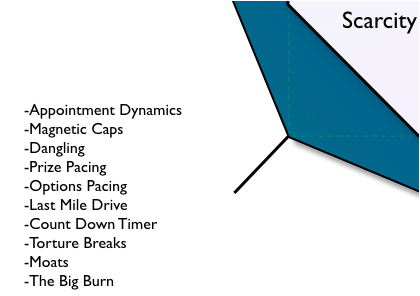
\includegraphics[scale=0.5]{img/chapter2/octalyst6.png}
\caption{Octalyst - niecierpliwo�� \cite{octalysis}}
\label{chapter2_octalyst6}
\end{figure} 

% =======================================
% nieprzewidywalnosc i ciekawosc

Innymi wa�nymi zasadami w systemie opartym na grywalizacji jest nieprzewidywalno�� oraz ciekawo�� (ang. \textit{Unpredictability}). Obie te zasady wykorzystuj� nieszkodliwe d��enie do tego, by dowiedzie� si�, co b�dzie dalej. Dla ludzkiego umys�u naturalnym stanem rzeczy jest my�lenie na temat, tego czego nie wiemy, a wiedzie� chcemy. Niestety nap�d ten jest te� g��wnym czynnikiem uzale�nienia od hazardu, gdy� jest podstaw� organizowania r�nych loterii. Przyk�adowe techniki wykorzystywane w tym obszarze s� widoczne na rysunku \ref{chapter2_octalyst7}, a na uwag� warto zwr�ci�, je�li chodzi o:

\begin{itemize}
\item Loteria - kluczowym za�o�eniem tej techniki jest zasada i� jak d�ugo pozostaniesz w grze, szanse na wygran� rosn�. Zazwyczaj mamy tutaj niski pr�g wej�cia oraz bardzo du�e nagrody, kt�rych szansa na wygran� jest bardzo niewielka i w du�ej mierze zale�y od szcz�cia. 
\item Easter Eggs - s� to niespodzianki przyznawane bez potwierdzenia przez u�ytkownika. Nagrody s� bardzo niskiej warto�ci, ale sam fakt powodzenia sprawia �e jest przyjemne do�wiadczenie. Dobrym przyk�adem tej techniki mog� by� ukryte wiadomo�ci od os�b tworz�cych dany system.
\item Mistyczne Skrzynki -  technika ta polega na organizowaniu w trakcie rozgrywki losowych nagr�d, kt�re s� wr�czane graczom po uzyskaniu zwyci�stwa. Uczucie jakie towarzyszy u�ytkownikowi podczas otwierania tytu�owej skrzynki jest bardzo zbli�one do tego, co czuj� dzieci podczas rozpakowywania prezent�w wigilijnych. 
\end{itemize}

\begin{figure}[H]
\centering
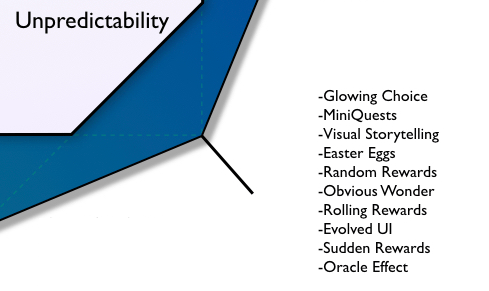
\includegraphics[scale=0.5]{img/chapter2/octalyst7.png}
\caption{Octalyst - nieprzewidywalno�� \cite{octalysis}}
\label{chapter2_octalyst7}
\end{figure} 

% =======================================
% unikanie strat

Ostatnim filarem wymienionym przez Chou jest unikanie strat (ang.  \textit{Avoidance}). Dotyczy ona unikania negatywnych zjawisk. Mo�e to by� zar�wno strata wykonanej pracy, jak i niemo�no�� wykonania dodatkowych zada�, kt�re mog� wymaga� wi�kszych nak�ad�w pracy.  Przyk�adowe techniki wykorzystuj�ce zasad� unikania strat s� widoczne na rysunku \ref{chapter2_octalyst8}, a najbardziej efektywne z nich s�:

\begin{figure}[ht]
\centering
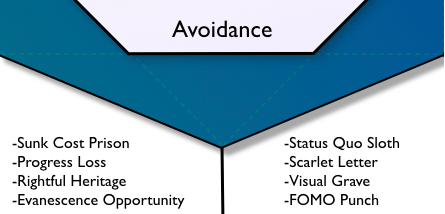
\includegraphics[scale=0.5]{img/chapter2/octalyst8.png}
\caption{Octalyst - unikanie strat \cite{octalysis}}
\label{chapter2_octalyst8}
\end{figure}

\begin{itemize}
\item Pe�noprawne dziedzictwo - technika ta polega na przekonaniu u�ytkownika, �e co� s�usznie nale�y do niego, a nast�pnie utwierdzeniu go w przekonaniu, �e je�li podejmie niepo��dane dzia�ania, to mo�e to straci�. 
\item Ulotna szansa - to technika polegaj�ce na motywowaniu u�ytkownika do szybkiego dzia�ania w obawie przez utrat� �wietnej oferty. �wietnie sprawdza si� tutaj wykorzystanie licznika czasu, kt�ry jeszcze bardziej zwi�ksza motywacj� u�ytkownika do skorzystania z oferty.
\item Sunk Cost Prison - nazwa tej techniki w j�zyku polskim nazywana jest wi�zieniem utopionych koszt�w. Jest on najbardziej wp�ywow� technik� zasady unikania strat. Wyst�puje w�wczas, gdy u�ytkownik mimo niech�ci, czy braku przyjemno�ci do wykonywania zada� dalej je realizuje, bo nie chce poczu� straty zwi�zanej z porzuceniem wszystkiego. Przyk�adem mo�e by� gra, kt�ra po wielu godzinach nam si� ju� znudzi�a, ale gramy w ni� dalej, bo nie chcemy porzuci� zdobytych w grze d�br. 
\end{itemize}


\section{Ochrona �rodowiska}

Pierwotnie aplikacja mia�a by� przeznaczona do kszta�towania w�r�d u�ytkownik�w wiedzy na temat ochrony �rodowiska i budowania w nich pozytywnych nawyk�w ekologicznych. Ostatecznie po konsultacjach zdecydowano si� na rozszerzenie systemu do mo�liwo�ci tworzenia kurs�w o dowolnej tematyce, zak�adaj�c, �e w ramach prac testowych zostanie utworzony kurs dotycz�cy w�a�nie ochrony �rodowiska. 


By w pe�ni zrozumie� potrzeby u�ytkownika konieczne by�o zapoznanie si� w�a�nie z t� tematyk�, bior�c pod uwag� materia� realizowany w szkole �redniej. Dzia� dotycz�cy ochrony �rodowiska mo�na podzieli� na 4 g��wne pod obszary:
\begin{itemize}
\item r�norodno�� biologiczna
\item zagro�enia bior�norodno�ci
\item sposoby ochrony przyrody
\item przeciwdzia�anie zanieczyszczeniom
\end{itemize}

% roznorodnosc biologiczna
\noindent R�norodno�� biologiczna to z definicji to rozmaito�� wszystkich organizm�w wyst�puj�cych na Ziemi oraz jest ona rozpatrywana na trzech poziomach organizacji �ycia \cite{biologia}: genetyczna, gatunkowa i ekosystemowa. R�norodno�� genetyczna oznacza zmienno�� przedstawicieli jednego gatunku wynikaj�c� z obecno�ci wielu alleli tego samego genu, dzi�ki temu przedstawiciele tego samego gatunku r�ni� si� wygl�dam, w�a�ciwo�ciami fizjologicznymi, czy zachowaniem. R�norodno�� gatunkowa polega z kolei na bogactwie wyst�puj�cych w danym ekosystemie gatunk�w. Ostatnim poziomem bior�norodno�ci jest bior�norodno�� ekosystemowa, czyli zr�nicowanie siedlisk i zamieszkuj�cych je organizm�w mierzone w liczb� wielogatunkowych zbiorowisk na danym obszarach.

Nale�y r�wnie� mie� na uwadze, �e r�norodno�� biologiczna zmienia si� w czasie - jedne gatunki wymieraj�, inne powstaj� lub zmieniaj� zasiedlane tereny. Wp�ywa to na wzrost lub malenie r�norodno�ci gatunkowej. Ze wzgl�du na wyst�puj�ce na naszej planecie r�nice klimatyczne w poszczeg�lnych regionach wyst�puj� obszary o du�ej r�norodno�ci biologicznej np. lasy tropikalne oraz takie o ma�ej np. tereny subpolarne. 

% zagrozenia bioroznorodnosci
Kolejnym obszarem poruszanym na lekcjach biologii w szkole �redniej s� zagro�enia bior�norodno�ci, z kt�rych g��wnym jest cz�owiek. Od momentu pojawienia si� cz�owieka skomplikowane zale�no�ci mi�dzy organizmami s� zaburzane przez jego dzia�alno��. Coraz cz�ciej prowadzi ona do nieodwracalnych zmian w �rodowisku. G��wn� przyczyn� spadku bior�norodno�ci jest niszczenie siedlisk czy nawet ca�ych ekosystem�w, na wskutek przekszta�cania tych teren�w pod obszary rolnicze, przemys�owe czy zurbanizowane. Nale�y mie� na uwadze, �e im bardziej intensywnie wykorzystywany jest dany obszar, to tym mniejsza jest na nim bior�norodno��.
Innym zagro�eniem dla bior�norodno�ci s� gatunki inwazyjne. Cz�owiek przemieszczaj�c si� w r�ne miejsca globu m�g� celowo lub przez przypadek przenie�� ze sob� r�ne organizmy. W nowych �rodowiskach s� one pozbawione swoich naturalnych wrog�w, wiec cz�sto wypieraj� rodzime gatunki. Obce gatunki nazywane s� w�wczas inwazyjnymi. Gatunki inwazyjne na terenie Polski to na przyk�ad:
\begin{itemize}
\item biedronka azjatycka - sprowadzona do Europy w celu walki z plag� mszycy, dzi� stanowi zagro�enie dla popularnej biedronki siedmiokropki, gdy� jako gatunek agresywny wygrywa z ni� walk� o terytorium i po�ywienie
\item szpak - sprowadzony do Stan�w Zjednoczonych, drastycznie zwi�kszy� swoj� populacj� i zagra�a rdzennym ameryka�skim gatunkom przez zajmowanie wi�kszo�ci dziupli 
\item barszcz Sosnowskiego - naturalnie wyst�powa� na Kaukazie, ale uda�o mu si� rozprzestrzeni� w Polsce w b�yskawicznym tempie, jest niezwykle trudny do zwalczenia i jego sok wywo�uje silne oparzenia 
\end{itemize}
Cz�owiek r�wnie� mo�e by� w pewnych przypadkach uznany za gatunek inwazyjny, gdy� konkuruje on z innymi gatunkami o zasoby �rodowiska. Poprzez swoj� dominacj� doprowadzi� on do drastycznego zmniejszenia drapie�nik�w, kt�re stanowi�y zagro�enia zar�wno dla zwierz�t hodowlanych, jak i samego cz�owieka. W przypadku rywalizacji o ro�liny cz�owiek r�wnie� wp�ywa na spadek bior�norodno�ci (t�pienie szkodnik�w). Cz�sto dzia�alno�� cz�owieka prowadzi do efektu kaskadowego, kiedy to zmniejszenie populacji jednego z gatunk�w wp�ywa na zmniejszenie, a nawet wygini�cie wielu innych. Bardzo dobrym przyk�adem jest tutaj wydra morska. W USA wydry morskie by�y masowo zabijane z powodu ich cennych sk�r, co skutkowa�o ich ma�� populacj�. Ma�a ilo�� wydr przy �yciu spowodowa�a wzrostu liczebno�ci je�owc�w, kt�re s� ich naturalnym pokarmem. Z kolei je�owce zjada�y coraz wi�cej mi�czak�w i glon�w, doprowadzaj�c do zmniejszenie r�norodno�ci gatunkowej i zaniku ��k podwodnych, kt�re poskutkowa�y wygini�ciem wielu gatunk�w ryb i bezkr�gowc�w, dla .kt�rych stanowi�y one schronienie i �r�d�o po�ywienia 

Kolejnym elementem sk�adowym wiedzy o ochronie �rodowiska jest ochrona przyrody.   Przyroda jak nieod��czna cz�� �rodowiska musi podlega� ochronie. Ze wzgl�du na zakres obj�tych ochron� element�w wyr�niamy ochron� indywidualn�, gatunkow� lub obszarow�. Istniej� r�wnie� podzia�y ochrony przyrody ze wzgl�du na zakres obj�tych ochron� element�w, stopie� ingerencji cz�owieka czy poziom ochrony. Na szczeg�ln� uwag� zas�uguj� tutaj formy ochrony obszarowej. W Polsce wyr�nia si� kilka ich rodzaj�w takich jak park narodowy, rezerwat przyrody, czy park krajobrazowy. 

Park narodowy to najwa�niejsza z wymienionych tutaj form ochrony, powo�ywana przez Rad� Ministr�w, obejmuje tereny niezmienione przez cz�owieka o powierzchni wi�kszej ni� 1000 ha i charakteryzuje si� szczeg�lnymi walorami przyrodniczymi, naukowymi, czy kulturowymi . Parki narodowe s� otoczone otulin�, kt�ra ma zabezpiecza� park przed zewn�trznymi zagro�eniami dzia�alno�ci cz�owieka. Rezerwat przyrody jest z kolei powo�ywany przez regionalnego dyrektora ochrony �rodowiska i stanowi teren niezmieniony lub zmieniony w ma�ym stopniu, mo�e by� cz�ci� parku narodowego i posiada� otulin�. W Polsce jest obecnie ponad 1400 rezerwat�w.  Ostatnia z form ochrony obszarowej to park krajobrazowy, kt�ry jest powo�ywany przez regionalnego dyrektora ochrony �rodowiska. Obejmuje du�y obszar, kt�ry podlega ochronie ze wzgl�du na walory przyrodnicze, krajobraz�w, czy ma du�e znaczenie rekreacyjne i edukacyjne, ze wzgl�du na infrastruktur� turystyczn� na jego terenie

% Przeciwdzia�anie zanieczyszczeniom

Opr�cz wymienionych wcze�niej form ochrony przyrody wa�ne jest r�wnie� racjonalne gospodarowanie zasobami przez cz�owieka w my�l zasady zr�wnowa�onego rozwoju. Dla cz�owieka najwa�niejszym tego aspektem jest przeciwdzia�anie zanieczyszczeniom �rodowiska. Mo�na to robi� poprzez recykling, korzystanie z odnawialnych �r�de� energii czy zmniejszenie emisji dwutlenku w�gla do atmosfery. 

We wsp�czesnym �wiecie energia elektryczna odgrywa bardzo wa�n� rol�. Ka�da gospodarka potrzebuje ogromnych nak�ad�w energii oraz ka�dy cz�owiek korzysta z niej na co dzie�. Zapewnienie wi�c odpowiednich �r�de� energii jest kluczowe.

Energetyka niekonwencjonalna (Rys. \ref{chapter2_energia}) rozwija si� na �wiecie od kilkudziesi�ciu lat. Rozw�j ten przybra� na sile w ostatnim czasie i mia�o to wiele przyczyn. Do g��wnych czynnik�w nap�dzaj�cych energetyk� niekonwencjaln� mo�na zaliczy� d��enie do lepszej ochrony �rodowiska, mniejsz� awaryjno�� czy rozw�j nowoczesnych rozwi�za� w tej dziedzinie. �mia�o mo�na stwierdzi�, �e kluczowym silnikiem nap�dzaj�cym rozw�j tych technologii by�o u�wiadomienie sobie nieuchronno�ci wyczerpywania si� zasob�w naturalnych takich jak w�giel, czy ropa naftowa.

\begin{figure}[H]
\centering
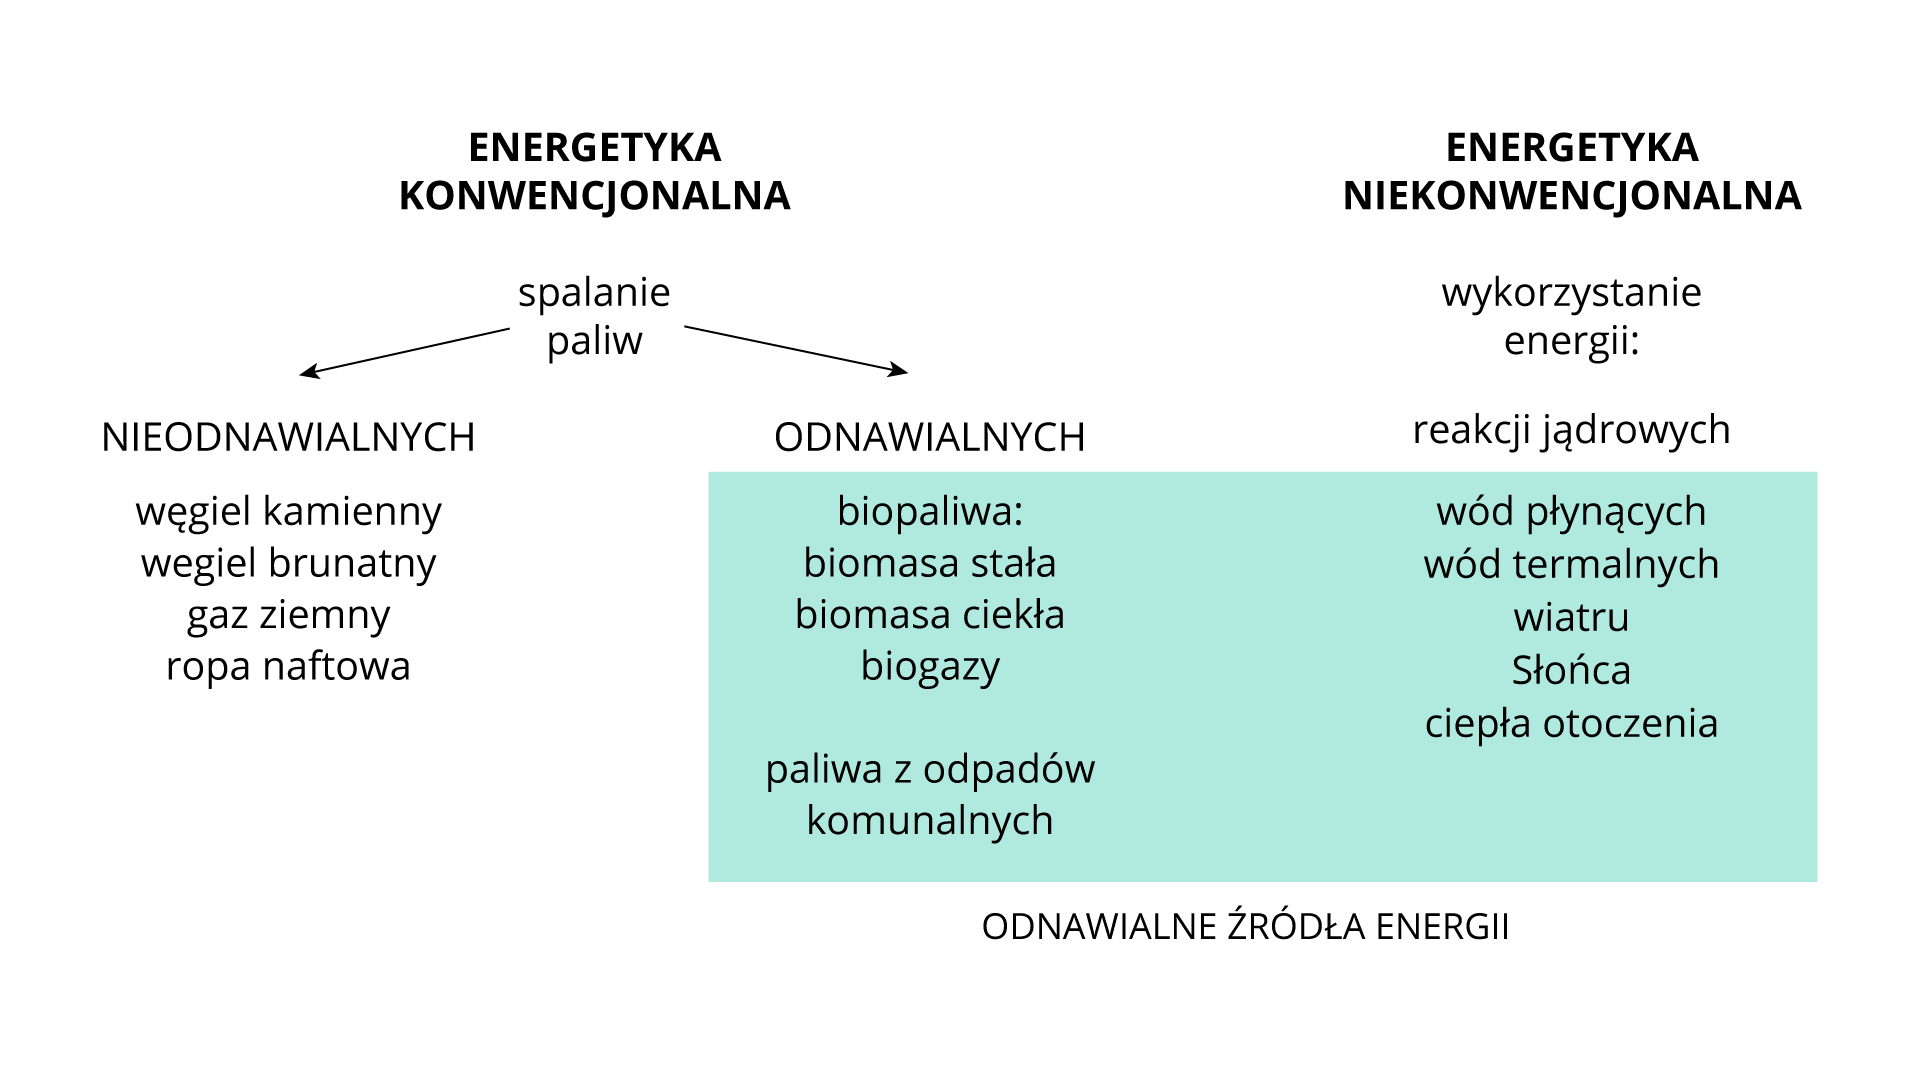
\includegraphics[scale=0.2]{img/chapter2/energia.png}
\caption{Podzia� �r�de� energii \cite{energia}}
\label{chapter2_energia}
\end{figure} 

Inny sposobem na racjonalne gospodarowanie zasobami przyrody jest recykling. Jego celem jest ograniczenie zu�ycia surowc�w naturalnych oraz zmniejszenie ilo�ci odpad�w. Recykling obejmuje odzyskiwanie surowc�w z produkt�w odpadowych i wykorzystywanie ich do produkcji nowych, poszukiwanych towar�w. Zasad� dzia�ania recyklingu jest maksymalizacja ponownego wykorzystania materia��w odpadowych, z uwzgl�dnieniem minimalizacji nak�ad�w na ich przetworzenie, przez co chronione s� surowce naturalne, kt�re s�u�� do ich wytworzenia oraz surowce s�u��ce do ich p�niejszego przetworzenia. Recykling odbywa si� w dw�ch obszarach: produkowania d�br oraz p�niejszego powstawania z nich odpad�w. Za�o�enia recyklingu zak�adaj� wymuszanie odpowiednich postaw producent�w d�br, sprzyjaj�cych produkcji materia��w jak najbardziej odzyskiwalnych oraz tworzenie odpowiednich zachowa� u odbiorc�w tych d�br. W recyklingu kluczow� rol� odgrywa segregacja odpad�w. Ma ona na celu usprawnienie zar�wno recyklingu materia��w wielokrotnego u�ytku oraz u�atwi� utylizacj� pozosta�ych odpad�w. Zgodnie za zasadami prawid�owej segregacji �mieci nale�y wrzuca� �mieci do odpowiednio oznaczonych pojemnik�w. 

\chapter{Przegl�d podobnych system�w}

Jednym z pierwszych krok�w tworzenia naszej aplikacji, by�o sprawdzenie czy w sieci nie
istniej� ju� aplikacje, podobne do naszej. Znaleziono wiele system�w, kt�re w r�nych stopniach zawiera�y planowane elementy naszej aplikacji, jednak�e nie uda�o si� znale�� niczego w du�ym stopniu podobnego. 

Wi�kszo�� istniej�cych aplikacji skupia si� na wybranych pojedynczych aspektach, z kt�rych planowo wi�kszo�� ma pojawi� si� w projektowanym systemie. Celem jest utworzenie takiego systemu, w kt�rym mo�na po��czy� elementy grywalizacji z przyjemnym sposobem nauczania i rozmaitymi, ciekawymi formami sprawdzania wiedzy. Dodatkowym atutem systemu mia�oby by� zapewnienie mo�liwo�ci kszta�towania nawyk�w zwi�zanych z dan� dziedzin�. Poni�ej przedstawiono istniej�ce systemy, kt�re wed�ug nas w dobrze spe�niaj� si� w obszarach, w kt�rych nasz system ma dzia�a�. 

\section{Habitica.com}

Habitica to aplikacja do zarz�dzania zadaniami online. W przeciwie�stwie do wi�kszo�ci
program�w do planowania czasu, Habitica ma form� gry fabularnej, przez co w
bardzo dobry spos�b wykorzystuje grywalizacj� do kszta�towania nawyk�w.
System ten u�o�ony w formie gry RPG, w kt�rej gracz zbiera przedmioty, takie jak z�oto i zbroja,
aby rozwija� swoj� posta�. Nagrody s� otrzymywane poprzez wykonywanie rzeczywistych
cel�w, w formie nawyk�w lub zada� do wykonania. 

Nawyki s� d�ugoterminowymi celami, kt�re s� wykorzystywane do zmiany nawyk�w danej
osoby. Mog� one by� ustawione jako pozytywne lub negatywne. Zadania do wykonania mog� by� w zdefiniowane jako jednorazowe lub dzienne. Zadania dzienne  to takie, kt�re u�ytkownik planuje wykonywa� ka�dego dnia. Zadania jednorazowe wykonuje si� tylko raz i znikaj� po ich zrealizowaniu. Za wykonanie negatywnego nawyku lub niezrealizowaniu zadania dziennego posta� traci punkty zdrowia, a  za wykonanie pozytywnych aktywno�ci gracz otrzymuje punkty do�wiadczenia oraz z�oto.

\begin{figure}[ht]
\centering
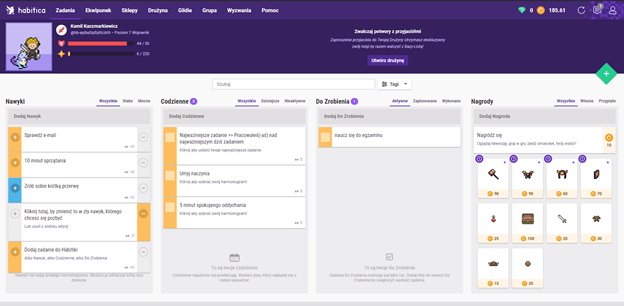
\includegraphics[scale=0.6]{img/chapter3/habitica.png}
\caption{Przyk�adowy widok na panel z zadaniami na Habitica.com}
\label{chapter3_habitica}
\end{figure}

Dzi�ki zdobytemu do�wiadczeniu i z�otu u�ytkownik mo�e rozwija� swoj� posta� poprzez kupowanie przedmiot�w i odblokowywanie nowych umiej�tno�ci. Dodatkowo gracze mog� tworzy� dru�yny, by wykonywa� te same zadania oraz bra� udzia� w wydarzeniach sezonowych, dzi�ki kt�rym mog� zdobywa� unikalne przedmioty. 

Aplikacja ta w �wietny spos�b wykorzystuje mechanizmy grywalizacji do motywowania u�ytkownika do realizowania zdefiniowanych przez niego zada�. Niestety nie ma w niej narz�dzi, kt�re pozwalaj� na weryfikacj� wykonanych zada� oraz przyswajanie nowej wiedzy. Mimo tego mo�e pos�u�y� jako wz�r dla naszej aplikacji w kontek�cie samej grywalizacji. Dodatkowo gracze mog� tworzy� dru�yny, by wykonywa� te same zadania oraz bra�
udzia� w wydarzeniach sezonowych. 

\section{Quizizz.com}

Quizizz jest systemem wykorzystywanym w klasach lub pracach grupowych. Pozwala on nauczycielom i uczniom razem pracowa� online w tym samym czasie. Wykorzystuje metod� nauczania i uczenia si� w stylu quizu, gdzie u�ytkownik odpowiada na seri� pyta� i rywalizuje z innymi u�ytkownikami w tym samym quizie.

Quizizz mo�e by� u�ywany jako narz�dzie "sprawdzaj�ce", kt�re pokazuje, jak studenci znaj� materia�. Nauczyciele mog� wykorzystywa� Quizizz do udost�pniania uczniom materia��w w formie na przyk�ad slajd�w, tworzenia test�w dla uczni�w oraz zadawania im prac domowych. Uczniowie po sprawdzeniu swojej wiedzy moj� dost�p do odpowiedzi, by w razie udzielenie niepoprawnych odpowiedzi, dowiedzie� si� jaka jest prawid�owa odpowied� na dane pytanie.

Aplikacja ta jest do�� prosta w u�yciu dla uczni�w i nauczycieli. Uczniowie mog� si� zarejestrowa� za pomoc� swojego konta Google lub konta na Facebook, a nast�pnie mog� zacz�� korzysta� z Quizizz. Nauczyciele po rejestracji wystarczy, �e klikn�  "utw�rz quiz" w g�rnej cz�ci strony, by rozpocz�� tworzenie pyta�.

\begin{figure}[ht]
\centering
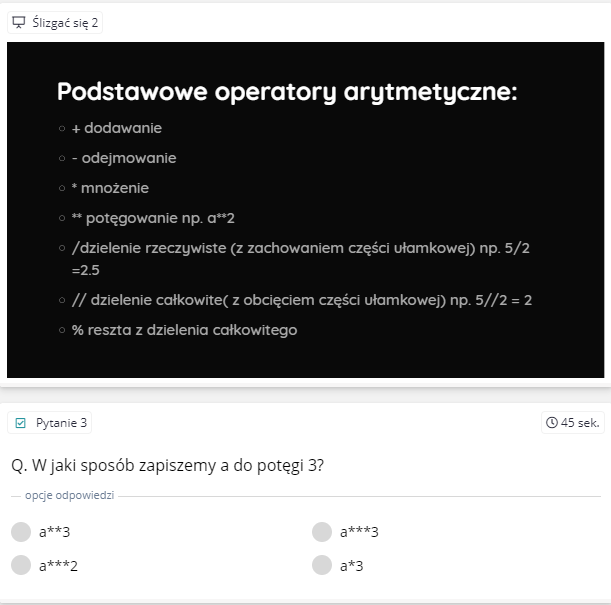
\includegraphics[scale=0.4]{img/chapter3/quizizz.png}
\caption{Przyk�adowe wygl�d quizu na Quizizz.com}
\label{chapter3_quizizz}
\end{figure}

System ten zawiera przejrzysty interfejs oraz jest �atwy w obs�udze. Jest dobr� aplikacj� do nauczania oraz sprawdzania wiedzy. Jednak�e w wi�kszo�ci s� to slajdy z informacjami dla uczni�w oraz quizy sprawdzaj�ce wiedz�. Docelowo w naszym systemie ma by� zapewniona wi�ksza r�norodno�� form sprawdzaj�cych wiedz�. Dodatkowo bardzo wa�nymi aspektami s� dla nas elementy grywalizacji oraz kszta�towania nawyk�w, kt�rych w tym systemie brakuje.

\section{Wordwall.net}

Wordwall jest aplikacj� pozwalaj�c� na sprawdzenie wiedzy z danej dziedziny poprzez rozwi�zanie r�norodnych �wicze�. Ma intuicyjny interfejs oraz jest bardzo prosty w obs�udze, co czyni go �wietnym rozwi�zaniem dla os�b nie radz�cych sobie najlepiej z technologi�.

Nauczyciel po przygotowaniu materia��w, z kt�rych chce sprawdzi� wiedz� swoich podopiecznych, mo�e utworzy� testy wykorzystuj�c gotowe szablony. Zaoszcz�dza dzi�ki temu du�o czasu oraz tak utworzone �wiczenia mog� by� wykonywane w wielu trybach.

\begin{figure}[ht]
\centering
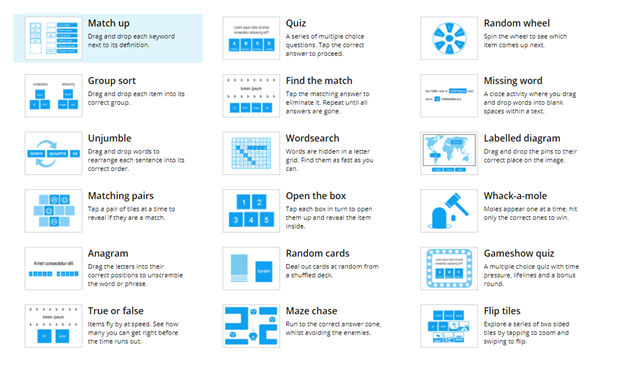
\includegraphics[scale=0.4]{img/chapter3/wordwall.png}
\caption{Przyk�adowe szablony zada� na Wordwall.net}
\label{chapter3_wordwall}
\end{figure}

Aplikacja ta pozwala na sprawdzeni swojej wiedzy na wiele sposob�w. Mo�na wydrukowa� zadania albo rozwi�za� je na urz�dzeniu z dost�pem do Internetu. W formie elektronicznej mam mo�liwo�� wybrania konkretnego szablonu. Przyk�adowe szablony przedstawione s� na rysunku \ref{chapter3_wordwall}. Nauczyciele w prosty spos�b mog� sprawdzi� wyniki swoich uczni�w, kt�rzy uko�czyli dane zadania.

Pomimo brak�w w  aplikacji w aspektach kszta�towania nawyk�w, grywalizacji i r�norodnego sposobu przekazywania wiedzy charakteryzuje si� ona niesamowit� r�norodno�ci� form sprawdzania wiedzy. Dodatkowo Wordwall pokazuje, �e robienie tak zr�nicowanych zada� mo�e by� proste i nie wymaga� wiele czasu od os�b uk�adaj�cych testy.

\section{Por�wnanie z projektem}

Po przegl�dzie podobnych system�w mo�na stwierdzi�, �e zazwyczaj specjalizuj� si� one w jednej kwestii. Przyk�adowo \textit{Habitica.com} g�ruje nad pozosta�ymi systemami w wykorzystaniu  mechanizm�w gamifikacji. Dodatkowym jej atutem jest mo�liwo�� pracy z nawykami poprzez budowania pozytywnych i neutralizowanie tych negatywnych. \textit{Wordwall.net} z kolei skupia si� w g��wnej mierze na aspektach przekazywania i sprawdzania wiedzy. W wytwarzanym systemie planem jest znale�� w�a�nie z�oty �rodek pomi�dzy tymi dziedzinami tj. wykorzystaniu gamifikacji do skonstruowania lepszych form sprawdzaj�cych wiedz�. 



\chapter{Analiza systemu (Marek Grudkowski)}

	\section{Wizja systemu}

\subsection{Interesariusze i ich problemy}

Minione kilkana�cie lat to okres dynamicznego rozwoju Internetu i globalizacja
informacji. Wraz z jego rozwojem pojawiaj� coraz to nowsze sposoby na
wykorzystanie jego zasob�w. Jednym z nich jest nauczanie na odleg�o��.
Pozwala ono na zg��bianiu tajnik�w r�nych dziedzin bez potrzeby fizycznego
kontaktu z osob� przekazuj�c� wiedz�.

Zdalne nauczanie sta�o si� bardzo g�o�nym tematem w ci�gu ostatniego roku,
czego przyczyn� jest �wiatowa pandemia korona wirusa. Wiele szk� zamkni�to i
nakazano przej�cie na nauczanie zdalne. Wa�nym pytaniem jest to, jak pandemia 
wp�yn�a zar�wno na rozw�j zdalnego nauczania pod wzgl�dem informatycznym, jak 
i na metody stosowane przez pedagog�w, kt�rzy gwa�townie z dnia na dzie� musieli 
zmieni� swoje codzienne nawyki pracy. G��wnym problem zwi�zanym z nauczaniem 
zdalnym jest prze�amanie barier edukacyjnych takich jak miejsce zamieszkania, 
sztywne pory zaj�� czy umiej�tno�� obs�ugi oprogramowania. W du�ej mierze 
prze�amanie owej bariery zale�y w g��wnie od ch�ci zdobycia wiedzy, a uczniem 
mo�e by� zar�wno dziecko, jak i osoba doros�a.

W okresie lockdownu wielu z uczni�w szk� podstawowych, ponadpodstawowych, czy 
nawet student�w traci�o zapa� do nauki. Wielu nauczycieli twierdzi, �e poprzez 
komputer trudno z uczeniem utworzy� wi�. Okazuje si� czym�, co zwi�ksza zaufanie 
i motywacje uczni�w do nauki. Problemem podczas nauki zdalnej jest te� 
nieprzystosowanie nauczycieli do prowadzenia  zaj�� w formie zdalnej. Wielu z 
nich posiada wspania�e materia�y, ale mog� je wykorzysta� tylko na zaj�ciach 
stacjonarnych. Brak odpowiednich umiej�tno�ci  technicznych oraz niska motywacja 
uczni�w znacz�co wp�ywaj� r�wnie� na to, jakie podej�cie ma nauczyciel. Te dwie
grupy - uczniowie i nauczyciele s� g��wnymi interesariuszami projektu.

Problemem u wi�kszo�ci nauczycieli jest s�aba znajomo�� oprogramowania 
wykorzystywanego podczas nauki zdalnej oraz brak skutecznych sposob�w motywowania 
uczni�w do chocia�by podj�cia pr�by nauki. Uczniowie potrzebuj� w�a�nie mechanizmu, 
kt�ry wytworzy� by w nich pozytywne nawyki oraz ch�� zdobywania wiedzy. Tutaj 
�wietnym rozwi�zaniem mo�e okaza� proponowana przez nas aplikacja, wykorzystuj�ce 
mechanizmy gamifikacji. 

\subsection{Proponowane rozwi�zanie}

Proponowane rozwi�zanie to aplikacja, na kt�rej nauczyciel b�dzie m�g�  tworzy� i realizowa� kursy dla swoich podopiecznych. Kursy takie dodatkowo, by  zach�ci� uczni�w do udzia�u w nich b�d� opiera� si� na mechanizmach gamifikacji. 
W ka�dym kursie nauczyciel b�dzie m�g� w prosty spos�b tworzy� aktywno�ci i monitorowa�, w kt�rych uczniowie b�d� mogli bra� udzia�. Aktywno�ci definiowane przez autora takiego kursu mo�na podzieli� na 3 grupy:
\begin{itemize}
\item zadania - zwyk�e zadania, na kt�re uczniowie przesy�aj� odpowiedzi, nauczyciel 
po sprawdzeniu wys�anego rozwi�zania przydziela jej autorowi odpowiedni� ilo�� punkt�w, 
je�li zadanie takie jest obowi�zkowe to mo�e odejmowa� punkty za nie wys�anie odpowiedzi
\item wydarzenia - jest to aktywno�� grupowa, kt�ra ma zmobilizowa� uczni�w do wsp�pracy; 
nauczyciel definiuje tutaj zestaw pyta� zamkni�tych, a uczniowie musz� odpowiedzie� na 
nie okre�lon� liczb� razy, dodatkowym aspektem jest to, �e odpowiedzi mo�na udziela� 
raz na jaki� czas
\item ciekawostki - nie mo�na tego nazwa� stricte aktywno�ci�, z za�o�enia maj� to by� 
notatki, przypomnienia, ciekawe fakty, kt�re b�d� si� wy�wietla� losowo uczestnikom kursu 
na zasadzie podobnej do reklam
\end{itemize}
Dla nauczyciela wa�ne jest te� monitorowanie tego, kto bierze udzia� w kursie i w 
jakim stopniu jest zaanga�owany. Dlatego konieczne jest r�wnie� wprowadzenie dla autora 
kursu panelu, kt�ry umo�liwia mu przegl�danie takich informacji, czy generowanie raport�w 
do szkolnej dokumentacji. 

Od strony ucznia aktywno�ci wygl�daj� zupe�nie inaczej. Ot� podczas do��czania do 
kursu ka�dy uczestnik otrzymuje swojego w�asnego bohatera, kt�rego musi rozwija� 
poprzez wykonywanie misji. Jako misje rozumiemy tutaj w�a�nie zadania, kt�re wcze�niej 
zosta�y zdefiniowane przez nauczyciela. Aplikacja ma zapewni� od strony ucznia, by uwa�a� 
on i�, wykonywanie tych zada� to nie wys�anie notatki z lekcji, lecz przyk�adowo walka z 
potworem, by awansowa� swoj� posta� na wy�szy poziom. Dla ucznia ca�y kurs powinien posiada� 
tak� otoczk�. Podczas rozwijania swojej postaci mo�e przydziela� jej wybrane przez siebie 
atrybuty oraz kupowa� dla niej przedmioty, a wydarzenia specjalne maj� zapewnia� tak wysokie 
nagrody, by prosili prywatnie swoich koleg�w i kole�anki z klasy, by pomogli im j� wygra�. 

\subsection{Wymagania funkcjonalne, jako�ciowe i ograniczenia}

Zar�wno nauczyciele jako autorzy kurs�w, jak i uczniowie jako ich uczestnicy maj� specyficzne
wymaganie dotycz�ce aplikacji. Podczas jej projektowania nale�y wzi�� pod uwag�, to w jakim
kontek�cie b�d� z niej korzysta�, co mo�e sprawi� problemy, a co mo�e utrudni� ich
wyst�pienie. Kluczowe w tym aspekcie s� wymagania funkcjonalne. S� to takie wymagania, kt�re dotycz� wyniku zachowania systemu, kt�ry powinien zosta� dostarczony przez funkcj� systemu. 

\begin{table}[h]
\caption{Wymagania funkcjonalne}
\label{chapter4_tab_funkcjonalne}
\centering
\begin{tabular}{|l|l|c|}
\hline
U�ytkownik & Funkcja & Priorytet \\ \hline

\multirow{12}{*}{\makecell{Nauczyciel \\ (autor kursu)}} 

	& Mo�liwo�� tworzenia kurs�w & 1
		\\ \cline{2-3} 
	& Mo�liwo�� wyboru otoczki fabularnej & 3         		
		\\ \cline{2-3} 
    & Mo�liwo�� zapraszania u�ytkownik�w & 1          	
    	\\ \cline{2-3} 
	& Kontakt z uczestnikami kursu & 2   
		\\ \cline{2-3} 
	& Mo�liwo�� tworzenia zada� & 1
		\\ \cline{2-3} 
	& Mo�liwo�� zapisywania szablon�w zada� & 2
		\\ \cline{2-3} 
	& Tworzenie wydarze� dla wszystkich uczestnik�w & 1
		\\ \cline{2-3} 
	& Funkcja do definiowania wy�wietlanych uczestnikom notatek & 2
		\\ \cline{2-3} 
	& Dost�p do rozwi�za� nades�anych przez uczestnik�w & 1
		\\ \cline{2-3} 
	& Podgl�d panelu aktywno�ci uczestnik�w & 2
		\\ \cline{2-3} 
	& Mo�liwo�� indywidualnego kontaktu z uczestnikami & 3
		\\ \cline{2-3} 
	& Dost�p do raport�w z przebiegu poszczeg�lnych zada� & 2
		\\ \hline
	

\multirow{8}{*}{\makecell{Ucze� \\ (uczestnik kursu)}} 
	
	& Mo�liwo�� do��czania do kurs�w & 1
		\\ \cline{2-3} 
	& Mo�liwo�� tworzenia postaci per kurs & 1
		\\ \cline{2-3} 
	& Mo�liwo�� rozwijania postaci & 1
		\\ \cline{2-3}
	& Dost�p do aktywno�ci, za kt�re s� nagrody & 1
		\\ \cline{2-3}
	& Dost�p do sklepu z przedmiotami dla postaci & 2
		\\ \cline{2-3}
	& Mo�liwo�� indywidualnego kontaktu z innymi uczestnikami & 3
		\\ \cline{2-3}
	& Dost�p do rankingu postaci w danym kursie & 3
		\\ \cline{2-3}
	& Dost�p do panelu z powiadomieniami & 2
		\\ \hline


\end{tabular}
\end{table}

Poza wymaganiami funkcjonalnymi w procesie projektowania nale�y r�wnie� wzi�� pod uwag�
wymagania jako�ciowe oraz ograniczenia, jakie mog� wyst�powa�. Wymaganie jako�ciowe to wymaganie, kt�re dotyczy jako�ci tworzonego oprogramowania, kt�re nie zosta�o okre�lone przez wymagania funkcjonalne \cite{wolskipro}. Ograniczenia r�wnie� s� r�wnie� wymaganiami. R�ni� si� one tym od poprzednich, tym �e po prostu ogranicza przestrze� rozwi�za� poza to, co zosta�o zdefiniowane w wymaganiach funkcjonalnych i jako�ciowych. 

Wymagania jako�ciowe zazwyczaj dzielone s� na kilka podgrup. W projektowanej aplikacji podzielono je w�a�nie w ten spos�b i wyodr�bniono 6 podstawowych kategorii:
\begin{itemize}
\item wydajno�� - mo�liwo�� jednoczesnego korzystania przez 1000 u�ytkownik�w
\item dost�pno�� - zak�adaj�c, �e zar�wno uczniowie, jak i nauczyciele mog� korzysta� aplikacji wsz�dzie, powinna ona by� dost�pna co najmniej 20 godzin na dob�
\item ochrona - zapewnienie bezpiecze�stwa danych osobowych uczestnik�w kursu i podj�tych przez nich w nim aktywno�ci 
\item przeno�no�� - dost�pno�� aplikacji z poziomu przegl�darki, zar�wno na komputerze, jak i urz�dzeniu mobilnym
\item elastyczno�� - na chwil� obecn� nie przewiduje si� gruntownych zmian w projekcie systemu, jednakowo� warto zostawi� w nim furtki na przysz�o��, kt�re pozwol� na dodawanie nowych funkcjonalno�ci takich jak np. system osi�gni�� 
\item konfigurowalno�� - mo�liwo�� definiowania otoczki fabularnej w kursie
\end{itemize} 
\vspace{0.3cm}
Ograniczenia wyodr�bnione podczas analizy projektu:
\begin{itemize}
\item czasowe - czas realizacji projektu to pocz�tek grudnia
\item konieczno�� dzia�ania w specyficznych warunkach - potrzebny jest dost�p do Internetu
\item okre�lone formaty danych - pobieranie szablon�w i raport�w w okre�lonych formatach danych (xls, csv, json)
\item dokumentacja - utworzenie wiki z dokumentacj� i wskaz�wkami dla u�ytkownik�w
\item spos�b wdro�enia - 2 tygodniowy okres pr�bny z jednym kursem o tematyce ekologii w klasie szko�y ponadpodstawowej
\end{itemize}

	\section{Model przypadk�w u�ycia}
	\section{Diagram klas}

Po opisaniu przypadk�w u�ycia kolejnym krokiem prac projektowych by�o wykonanie diagramu klas. Jest to statyczny diagram, kt�rego celem jest przedstawi� struktur� systemu za pomoc� paradygmatu programowania obiektowego. W diagramie takim znajduj� si� poszczeg�lne klasy wraz ze swoimi atrybutami i metodami oraz zaznaczone zwi�zki i relacje pomi�dzy nimi\cite{klasyuml}. Zaprojektowany dla tworzonego systemu diagram klas mo�na zobaczy� na rysunku nr. \ref{chapter4_class}. Opis poszczeg�lnych klas jest dost�pny w tabeli nr. \ref{chapter4_classtable}. 

\begin{table}

% metadane tabeli
\caption{Opis klas przedstawionych na diagramie klas}
\label{chapter4_classtable}

\begin{tabular}{|p{3cm}|p{11cm}|}

\hline 
% naglowek
\textbf{Nazwa} & \textbf{Dokumentacja}\\\hline
% poczatek 1 wiersza
\vspace{0.1 mm} U�ytkownik & \vspace{0.1 mm}
Obiekty tej klasy to u�ytkownicy systemu. Powinni mie� mo�liwo�� logowania, wylogowania oraz zmiany ustawie� konta. 
\\
\vspace{0.1 mm} & \vspace{0.1 mm}
\\\hline
% koniec 1 wiersza

% poczatek 2 wiersza
\vspace{0.5px} Uczestnik & \vspace{0.5px}
Obiektem tej klasy jest u�ytkownik, kt�ry do��czy� do jednego z kurs�w. Dziedziczy w�a�nie od klasy U�ytkownik. 
\\
\vspace{0.2px} & \vspace{0.2px}
\\\hline
% koniec 2 wiersza

% poczatek 3 wiersza
\vspace{0.5px} Posta� & \vspace{0.5px}
Dla ka�dej instancji klasy Uczestnik zostaje przypisany jeden obiekt tej klasy. Reprezentuje on awatar uczestnika, kt�ry b�dzie rozwijany w miar� wykonywania przez niego zada�.  
\\
\vspace{0.2px} & \vspace{0.2px}
\\\hline
% koniec 3 wiersza

% poczatek 4 wiersza
\vspace{0.5px} Przedmiot & \vspace{0.5px}
Obiekty tej klasy mog� by� zbierane przez gracza w formie kolekcji. S�u�� do podnoszenia statystyk postaci. 
\\
\vspace{0.2px} & \vspace{0.2px}
\\\hline
% koniec 4 wiersza

% poczatek 5 wiersza
\vspace{0.5px} Kurs & \vspace{0.5px}
Klasa reprezentuj�ca kursy tworzone przez u�ytkownik�w. Posiada jednego autora oraz wielu uczestnik�w. 
\\
\vspace{0.2px} & \vspace{0.2px}
\\\hline
% koniec 5 wiersza

% poczatek 6 wiersza
\vspace{0.5px} Akywnosc & \vspace{0.5px}
Abstrakcyjna klasa, kt�ra stanowi punkt wyj�cia dla takich klas jak Wydarzenie, Zadanie, czy Pytanie. Po��czona agregacj� z klas� Kurs.  
\\
\vspace{0.2px} & \vspace{0.2px}
\\\hline
% koniec 6 wiersza

% poczatek 7 wiersza
\vspace{0.5px} Nawyk & \vspace{0.5px}
Klasa ta dziedziczy od Aktywno�ci. Reprezentuje zadania, kt�re maj� wyrobi� w uczestnikach danego kursu pozytywne nawyki.
\\
\vspace{0.2px} & \vspace{0.2px}
\\\hline
% koniec 7 wiersza

% poczatek 8 wiersza
\vspace{0.5px} Pytanie & \vspace{0.5px}
Klasa ta dziedziczy od Aktywno�ci. Obiekt tej klasy ma reprezentowa� pytania zamkni�te zadawane podczas wydarzenia. 
\\
\vspace{0.2px} & \vspace{0.2px}
\\\hline
% koniec 8 wiersza

% poczatek 9 wiersza
\vspace{0.5px} Zadanie & \vspace{0.5px}
Klasa ta dziedziczy od Aktywno�ci. Klasa ta reprezentuje zadania wykonywane przez uczestnik�w w trakcie kursu.  
\\
\vspace{0.1px} & \vspace{0.1px}
\\\hline
% koniec 9 wiersza

% poczatek 10 wiersza
\vspace{0.5px} Wydarzenie & \vspace{0.5px} 
Klasa ta dziedziczy od Aktywno�ci. Reprezentuje wydarzenia organizowane w trakcie kursu. Zawiera w sobie kolekcj� obiekt�w klasy Pytanie. 
\\
\vspace{12px} & \vspace{12px}
\\\hline
% koniec 10 wiersza

% poczatek 11 wiersza
\vspace{0.5px} Odpowiedz & \vspace{0.5px}
Klasa reprezentuj�ca odpowied� w wybranej aktywno�ci. Musi mie� przypisanego zar�wno autora (Uczestnik) jak i zadanie (Aktywno��). 
\\
\vspace{0.2px} & \vspace{0.2px}
\\\hline
% koniec 11 wiersza
\end{tabular}
\end{table}


\begin{figure}[ht]
	\centering
	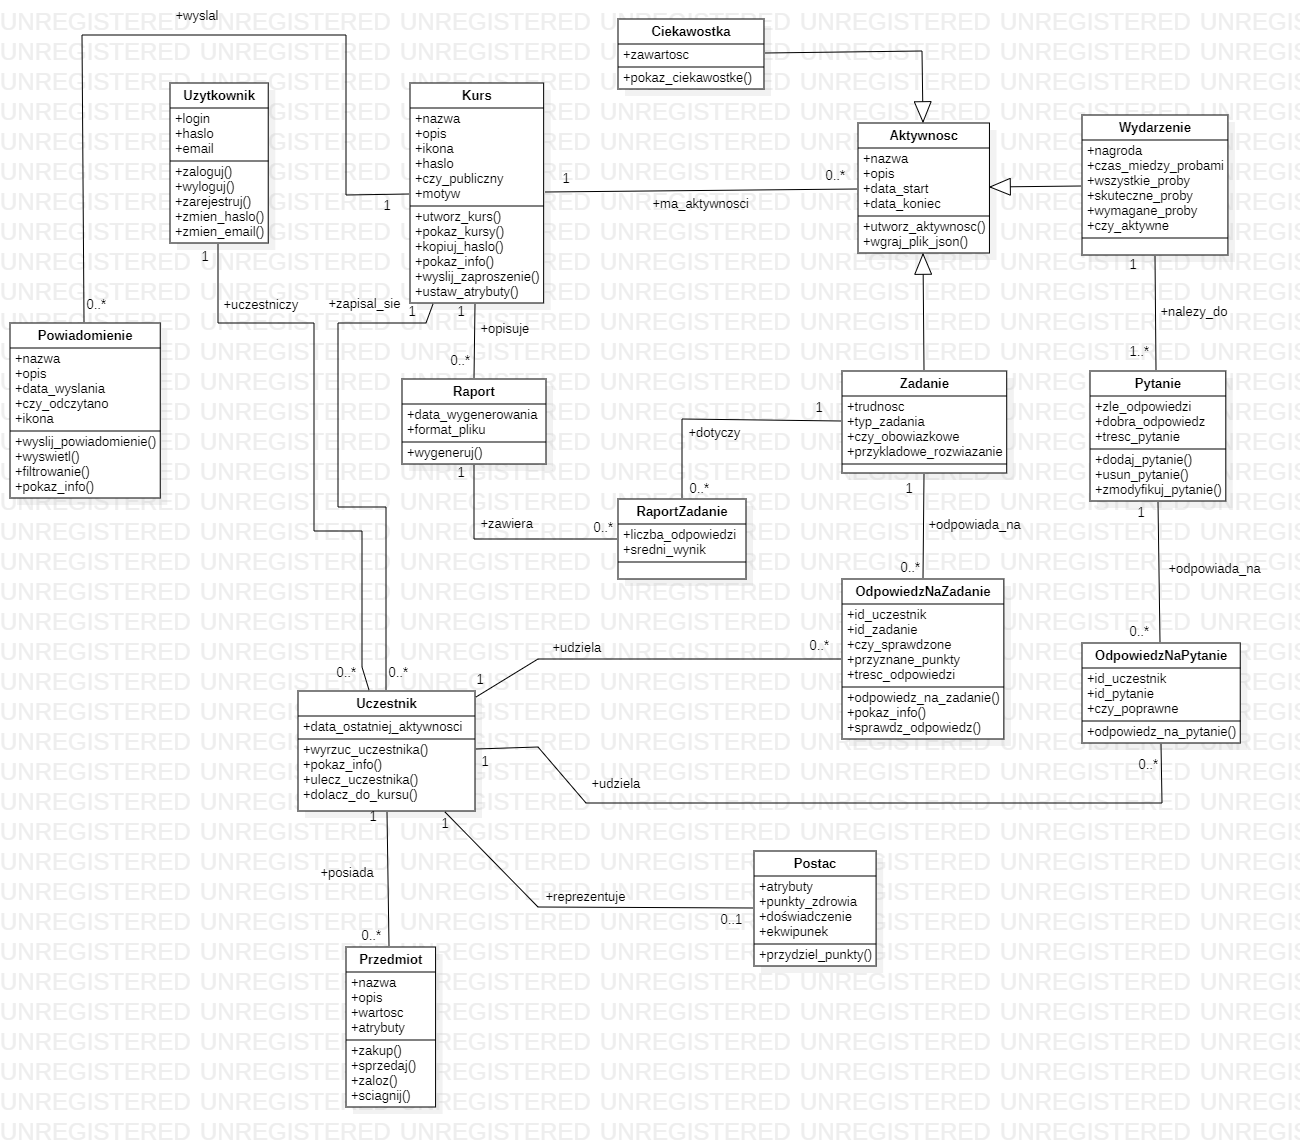
\includegraphics[width=1.3\textwidth, angle =90 ]{img/chapter4/class_diagram.png}
	\caption{Diagram klas}
	\label{chapter4_class}
\end{figure}
\chapter{Zagadnienia projektowo-implementacyjne}

Po analizie projektowanego systemu wybrano technologie i rozwi�zania, z kt�rych zesp� b�dzie korzysta� podczas jego implementacji. W przypadku stosowanych rozwi�za� postanowiono w g��wnej mierze opiera� si� na kulturze DevOps i jej rozbudowanych ideach. Je�li chodzi o wykorzystane technologi� system mia� by� zbudowany w oparciu o dwie technologie. Frontend mia� zosta� zbudowany w oparciu o framework React napisany w j�zyku Javascript. Z kolei do backendu mia� zosta� wykorzystany Django - framework napisany w j�zyku skryptowym Python. Aktualnie s� to technologie wysoce popularne na rynku i oferuj�ce wiele rozbudowanych mo�liwo�ci w tworzeniu serwis�w internetowych. 
	\section{Wybrane Rozwi�zania}

W tym podrozdziale om�wiono organizacj� pracy podczas implementacji systemu oraz wykorzystywane rozwi�zania. W g��wnej mierze wszystkie za�o�enia opieraj� si� na kulturze DevOps. Jest to metodyka pracy lub inaczej zestaw praktyk, kt�rych celem jest automatyzacja i integracja pracy wykonywanej przez programist�w w danym zespole \cite{devopsdef}. DevOps jest na tyle uniwersalnym rozwi�zaniem, �e ��czy w sobie cechy podej�cia zar�wno kaskadowego (\textit{Waterfall}), jak i zwinnego (\textit{Agile}).

Podczas prac implementacyjnych g��wny nacisk postawiono jedn� z podstawych zasad DevOps, jak� jest ci�g�a integracja (\textit{Continous Intergration}). W zwi�zku z tym utworzono repozytorium systemu kontroli wersji GIT na platformie Github. Pozwala ona w �atwy spos�b na wersjonowanie kodu �r�d�owego aplikacji oraz zaprojektowanie akcji, kt�re uruchamiane s� w zale�no�ci od rodzaju wprowadzonych zmian do kodu. 

\subsection{Praca z repozytorium}

Na g��wnej ga��zi repozytorium znajdowa� si� najnowszy kod �r�d�owy aplikacji, kt�ry zosta� zatwierdzony przez pozosta�ych cz�onk�w zespo�u. Przy wprowadzaniu nowych funkcjonalno�ci osoba odpowiedzialna za jej implementacj� tworzy�a osobn� ga���, z kt�rej wystawia�a na portalu Github pro�b� o po��czenie jej g��wn� ga��zi� (\textit{Pull Request}). 

Po wystawieniu takiej pro�by w ramach kultury DevOps pozostali cz�onkowie zespo�u  przeprowadzali przegl�d kodu w celu zapoznania si� z now� funkcjonalno�ci� i wskazaniu autorowi ewentualnych zmian w kodzie w celu zwi�kszenie jego czytelno�ci \cite{cleancode, pragmatyczny}. 

\subsection{Ci�g�a integracja}

Opr�cz przegl�du kodu przy wystawaniu pro�by o przy��czenie w�asnej ga��zi portal Github uruchamia� zaprojektowane przez zesp�l akcje, kt�rych celem jest analiza kodu pod wzgl�dem czytelno�ci oraz poprawno�ci. Akcje te zosta�y zaprojektowane przy wykorzystaniu technologii Docker Compose, kt�ra umo�liwia uruchamianie r�nych polece� na wirtualnych maszynach dostarczanych przez portal Github \cite{githubakcje}. W przypadku tworzonej aplikacje zaprojektowany ci�g akcji sk�ada� si� z 5 podstawowych polece�:
\begin{itemize}
\item nadanie etykiety dla zg�oszonej pro�by przy��czenia ga��zi
\item wykrycie w jakich miejscach kodu �r�d�owego wyst�pi�y zmiany w zg�oszonej pro�bie przy��czenia ga��zi, na podstawie tego polecenia dzia�aj� nast�pne
\item kompilacja kodu �r�d�owego dokumentacji w celu wygenerowania gotowej dokumentacji w postaci dost�pnej do pobrania jako artefakt, kod �r�d�owy akcji mo�na zobaczy� na listingu nr \ref{latexworkflow}
\item uruchomienie sprawdzenia zgodno�ci formatowania kodu �r�d�owego backendu w og�lnodost�pnymi standardami oraz poprawno�ci kodu, kod �r�d�owy akcji mo�na zobaczy� na listingu nr \ref{backendworkflow}
\item uruchomienie sprawdzenia zgodno�ci formatowania kodu �r�d�owego frontendu w og�lnodost�pnymi standardami oraz poprawno�ci kodu
\end{itemize}
\noindent
Poni�ej przedstawiono przyk�adowe fragmenty zaprojektowanych polece� wraz z komentarzami:
 
\lstset{style=python}
\begin{lstlisting}[caption={Akcja kompilowania dokumentacji}, label=latexworkflow]
build_latex:
    # Kontener na kt�rym b�dzie wykonywana akcja
    runs-on: ubuntu-latest
    # Informacja jakich akcji potrzebuje ta akcja �eby dzia�a�a mog�a si� uruchomi�
    needs: changes
    # Uruchom tylko, je�li pro�ba o przy��czenie ma etykiet� `docs`
    if: ${{ needs.changes.outputs.docs == 'true' }}
    steps:
    	# Krok: Pobranie repozytorium na maszyn�
      - name: Set up Git repository
        uses: actions/checkout@v2
    	# Krok: Kompilacja dokumentu LaTeX
      - name: Compile Latex document
        uses: xu-cheng/latex-action@v2
        # wskazanie g��wnego dokumentu
        with:
            root_file: docs/project/main.tex
        # wskazanie plik�w pomocniczych        
        env:
            TEXINPUTS: ".:./docs/project//:"
    	# Krok: Utworzenie zmiennej �rodowiskowej zawieraj�cej hash danej zmiany
      - name: Add short hash to distinguish commits
        run: echo "sha=`echo ${{github.event.pull_request.head.sha}}`" >> $GITHUB_ENV
    	# Krok: Udost�pnienie pliku pdf do pobrania jako artefakt
      - name: Upload Artifact 
        uses: actions/upload-artifact@v2
        with:
            name: docs-${{github.actor}}-${{github.event.number}}-${{env.sha}}
            path: main.pdf
\end{lstlisting}

\begin{lstlisting}[caption={Akcja sprawdzenia jako�ci kodu w j�zyku Python}, label=backendworkflow]
python_check:
    # Kontener na kt�rym b�dzie wykonywana akcja
    runs-on: ubuntu-latest
    # Informacja jakich akcji potrzebuje ta akcja �eby dzia�a�a mog�a si� uruchomi�
    needs: changes
    # Uruchom tylko, je�li pro�ba o przy��czenie ma etykiet� `backend`
    if: ${{ needs.changes.outputs.backend == 'true' }}
    steps:
    	# Krok: Pobranie repozytorium na maszyn�
      - name: Set up Git repository
        uses: actions/checkout@v2
    	# Krok: Pobranie Python na maszyn�
      - name: Set up Python
        uses: actions/setup-python@v2
        with:
          python-version: '3.x'
    	# Krok: Pobranie pakietu do sprawdzenia jako�ci kodu
      - name: Install black
        run: |
          python -m pip install --upgrade pip
          pip install isort black
    	# Krok: Uruchomienie sprawdzenia jako�ci kodu
      - name: Run black
        run: |
          black --check .
\end{lstlisting}
	\section{Architektura systemu (Kamil Kaczmarkiewicz)}

Projektowany system zosta� wykonany w oparciu o dwie technologie, z kt�rych pierwsza z nich odpowiada za logik� biznesow�, a druga za wygl�d aplikacji po stronie u�ytkownika. Pomi�dzy odpowiednimi komponentami ustanowiono spos�b komunikacji przedstawiony na rysunku nr \ref{chapter5_arch1}.


\begin{figure}[H]
	\centering
	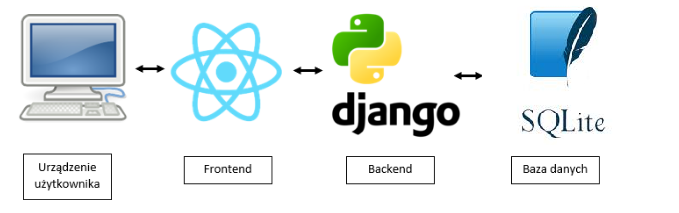
\includegraphics[scale=0.8]{img/chapter5/architektura_1.png}
	\caption{Architektura systemu}
	\label{chapter5_arch1}
\end{figure}

Docelowo poszczeg�lne komponenty mia�y zosta� umieszczone w kontenerach z wykorzystaniem technologii Docker, aby �atwo mo�na by�o umie�ci� je na serwerze. W�wczas model systemu zosta�by dodatkowo rozszerzony o dodatkowy komponent (serwer Nginx) odpowiedzialny za komunikacj� pomi�dzy komponentami na serwerze oraz obs�ug�  certyfikat�w (Rys. \ref{chapter5_arch2}). 

\begin{figure}[H]
	\centering
	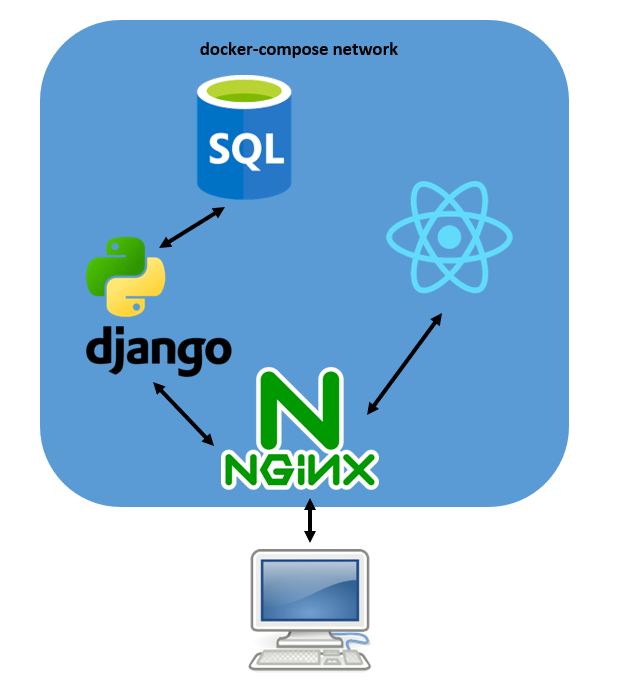
\includegraphics[scale=0.6]{img/chapter5/architektura_2.png}
	\caption{Architektura systemu z wykorzystaniem technologii Docker}
	\label{chapter5_arch2}
\end{figure}

Interfejs u�ytkownika powsta� w oparciu o bibliotek� typu open source napisan� w j�zyku Javascript - React. Jest to technologia, kt�ra  ��czy w sobie Javascript oraz znaczniki HTML w j�zyk nazywany JSX. 

G��wn� zalet� tej technologii jest mo�liwo�� definiowania komponent�w, kt�re reprezentuj� powtarzalne fragmenty stron internetowych takich jak stopka, czy nag��wek. Zasad� dzia�ania s� one zbli�one do klas w paradygmacie programowania obiektowego. Inn� kluczow� zalet� tego narz�dzia jest dynamiczne zarz�dzanie stanem strony i obiektowym modelem strony (ang. \textit{DOM}). Oznacza to �e w pami�ci powstaje struktura strony internetowej i w momencie zmianu stanu React podmienia tylko te cz�ci strony, kt�re tego wymagaj�.

Logika biznesowa zosta�a zaimplementowana w j�zyku skryptowym Python z wykorzystaniem narz�dzia Django. Django jest wysokopoziomowym web frameworkiem umo�liwiaj�cym tworzenie stron internetowych. Django zapewnia bardzo du�o wsparcie zwi�zane z tematem bezpiecze�stwa serwisu oraz pozwala na �atwe skalowanie projektu.

Django pozwala r�wnie� utworzy� instancj� relacyjnej bazy danych - SQLite - z kt�r� w bardzo prosty spos�b mo�e si� po��czy�, a nast�pnie na podstawie kodu napisanego z wykorzystaniem klas i obiekt�w jest w stanie je mapowa� na tabele w bazie danych. Umo�liwia r�wnie� wystawianie dla innych aplikacji punkt�w ko�cowych (ang. \textit{endpoint}), przez kt�re inne aplikacje wysy�aj� ��dania. Django obs�uguje dane ��dania przy wykorzystaniu informacji z bazy danych i zwraca odpowiedni� odpowied�. 
	\section{Projekt bazy danych (Krzysztof Sajko)}
\chapter{Zagadnienia implementacyjne}

	\section{Przyk�adowy podrozdzia�}

Tutaj opisujemy szczeg�y implementacji danej cz�ci systemu.

\chapter{Studium przypadku}

\chapter{Podsumowanie}



% ---------------------- Bibliografia -----------------------
\bibliographystyle{plain}                       % styl bibliografii
\begin{thebibliography}{3}                      % pocz�tek �rodowiska
\addcontentsline{toc}{chapter}{Wykaz literatury}    % dodaje bibliografi� do spisu tre�ci
\small              % spisy i bibliografie sk�adamy mniejszym stopniem pisma


% rodwald gamifikacja
\bibitem{rodwald}
Rodwald P.: \emph{Gamifikacja � czy to dzia�a?}, EduAkcja. Magazyn edukacji
elektronicznej nr 1 (11)/2016, str. 43�50 

% deterging gamifikacja
\bibitem{deterding}
Deterding S., Dixon D., Khaled R., Nacke L: \emph{From game design elements to
gamefulness: defining gamification}, Proceedings of the 15th International Academic
MindTrek Conference: Envisioning Future Media Environments, Tampere, Finland,
ACM, September 28-30, 2011, 9�15

% mochocki gamifikacja
\bibitem{mochocki}
Mochocki M.: \emph{Gamifikacja szkolnictwa wy�szego - obce wzorce, polskie perspektywy}, Game Industry Trends, Warszawa 2012

% link gamifikacja
\bibitem{octalysis}
Octalysis Complete Gamification Framework, https://yukaichou.com/gamification-examples/octalysis-complete-gamification-framework/ (data dost�pu 20.05.2021 r.).
  
% podrecznik biologia
\bibitem{biologia}
Bonar E., Krzeszowiec-Jele� W., Czachorowski S.: \emph{Biologia na czasie. Podr�cznik dla szk� ponadgimnazjalnych. Zakres Podstawowy.}, Nowa Era, Warszawa 2012

% platforma edukacyjne men
\bibitem{energia} Platforma edukacyjna MEiN, https://zpe.gov.pl/a/zrodla-energii-w-polsce/DZ9m3Dvd0/ (data dost�pu 12.06.2021 r.).

% wolski wymagania jakosciowe
\bibitem{wolskipro}
Blog dotyczacy modelowania UML, M. Wolski, https://wolski.pro/ (data dost�pu 12.09.2021 r.).

% bobkowska wyk�ady
\bibitem{usecase}
Model przypadk�w u�ycia, materia�y wyk�adowe z przedmiotu In�ynieria Oprogramowania, A. Bobkowska, Katedra In�ynierii Oprogramowania, Politechnika Gda�ska, 2020 r. 

% rup package use case
\bibitem{caseuse}
Rational Unified Process. Artifacts, https://sceweb.uhcl.edu/helm/RationalUnifiedProcess/, (data dost�pu 03.10.2021 r.)

% diagram klas 
\bibitem{klasyuml}
Diagramy klas UML, K. Tybulec, https://www.p-programowanie.pl/uml/diagramy-klas-uml (data dost�pu 18.10.2021 r.).

\end{thebibliography}                           % koniec �rodowiska % dodanie pliku bibliografii
% -----------------------------------------------------------

%------------------------------------------------------------
%	Dodanie wykazu rysunkow oraz tabeli

\renewcommand{\baselinestretch}{1.0}\normalsize	% interlinia w sekcji wykazow
\addcontentsline{toc}{chapter}{\listfigurename}	% dodanie wykazu rysunkow do spisu tresci
\listoffigures									% generacja wykazu rysunkow

\addcontentsline{toc}{chapter}{\listtablename}	% dodanie wykazu tabel do spisu tresci
\listoftables									% generacja wykazu tabel
\renewcommand{\baselinestretch}{1.3}\normalsize	% powrot do interlinii 1.5


% ---------------------- DODATKI -----------------------
% \chapter*{Dodatek A}
% \addcontentsline{toc}{chapter}{Dodatek A}
% \includepdf{dodatki/dodatek1.pdf}

% -----------------------------------------------------------
\end{document}
%------------------------------------------------------------
			 	%	Koniec pracy dyplomowej  %
%------------------------------------------------------------
